\chapter{Background \& Objectives}
Before commencing the design of the application and the project planning, it is important to have analysed what is hope to have been achieved at the end of the project time, and also what steps will need to be taken to implement each feature. As this report will mention later, choosing the best fitting life cycle methodology will play a big part of how the project will be shaped and how to create each feature whether it be by priority, size or difficulty. This section details the understandings for the project requirements, steps that are going to be needed to take, and as it would preferred that the project to is similar to an FDD one; developing an overall model and building the list of requirements and features.

\section{Background}
The choice of undertaking a project such as this one was due to two combining factors: maths and an interest to learn graphical programming. The fact that this application will require the learning graphics, and how to implement visual effects representing the requirements of the project in ways completely new in terms of a skill. As graphics is something the author have not had much to do with in the past, this project appears both exciting and daunting task due to the learning curve that will be needed to be taken. As for the maths factor, it can be assumed that quite a lot of maths will be involved(especially for creating curves, rolls and turns along most of the manoeuvres) which should be enjoyable to learn about.

As an individual currently studying for a degree in software engineering, a project that broadened the skill set from simply programming to graphics was another reason for choosing this topic. Rather than just coding a back-end web application, dealing with the visual side of an application is a new skill that could be gained from performing a project such as this one. Gains in time management and in writing a expansive report detailing findings and more importantly issues is something that will come from creating this project. 

In terms of the history of the topic, OLAN was originally developed by Michael Gorden in 2006\cite{Olan_Intro} and was designed to provide shorthand notation for pilots planning out aerobatic routines without having to draw out the full Aresti diagrams. In recent years, the OLAN notation became used much more until because of licensing issues with the original owner was taken off-line. Because of this, a new form of the notation has been created in a more open source way paving the way for applications such as this project's intended aim. Although in this report and the planned application itself will be still referring the notation as OLAN, the new re-make of the language is known as the 'OpenAero language'\cite{OpenAero_Language}. This is based off of the original, yet is open and allows anyone to use it. In combination with this, the creators of the OpenAero language also developed a web-based application\cite{OpenAero_Application} that allows the conversion of the notations to 2D Aresti diagrams. This is somewhat similar to what is hoped to have achieved, but alongside plenty more features most importantly the ability to see a plane perform the moves.

As for Aresti, named after its conceiver José Luis Aresti Aguirre\cite{Aresti} is the diagram format that OLAN achieves, and represent informative diagrams showing the shape of the routine, direction of travel, rolls and sharpness of turns. Aresti diagrams also can include angles or turns, ranging from 90 degrees to 270. Each diagram usually has a name\cite{Aresti_Simple}, relating normally to the shape of the manoeuvre, though some are more commonly known to pilots rather than the regular user. The OLAN notation for each diagram usually attempts to try describe the manoeuvre with the letter used, such as 'o' for a loop, or 'z' for a shark tooth. The full list of manoeuvres, including their OLAN notation and full name can be found on the OpenAero\cite{OpenAero_Language} site.

Upon starting this project, several meetings with the project supervisor are planned each providing more detail of the initial requirements. The project plan considering the requirements has been made into a rough Gantt chart which can be found in section~\ref{app:gantt1} of appendix A showing the plan following. Because several meetings have already happened at this stage, a fairly accurate time-scale to work with can be provided.\\

\begin{figure}[h!]
  \centering
      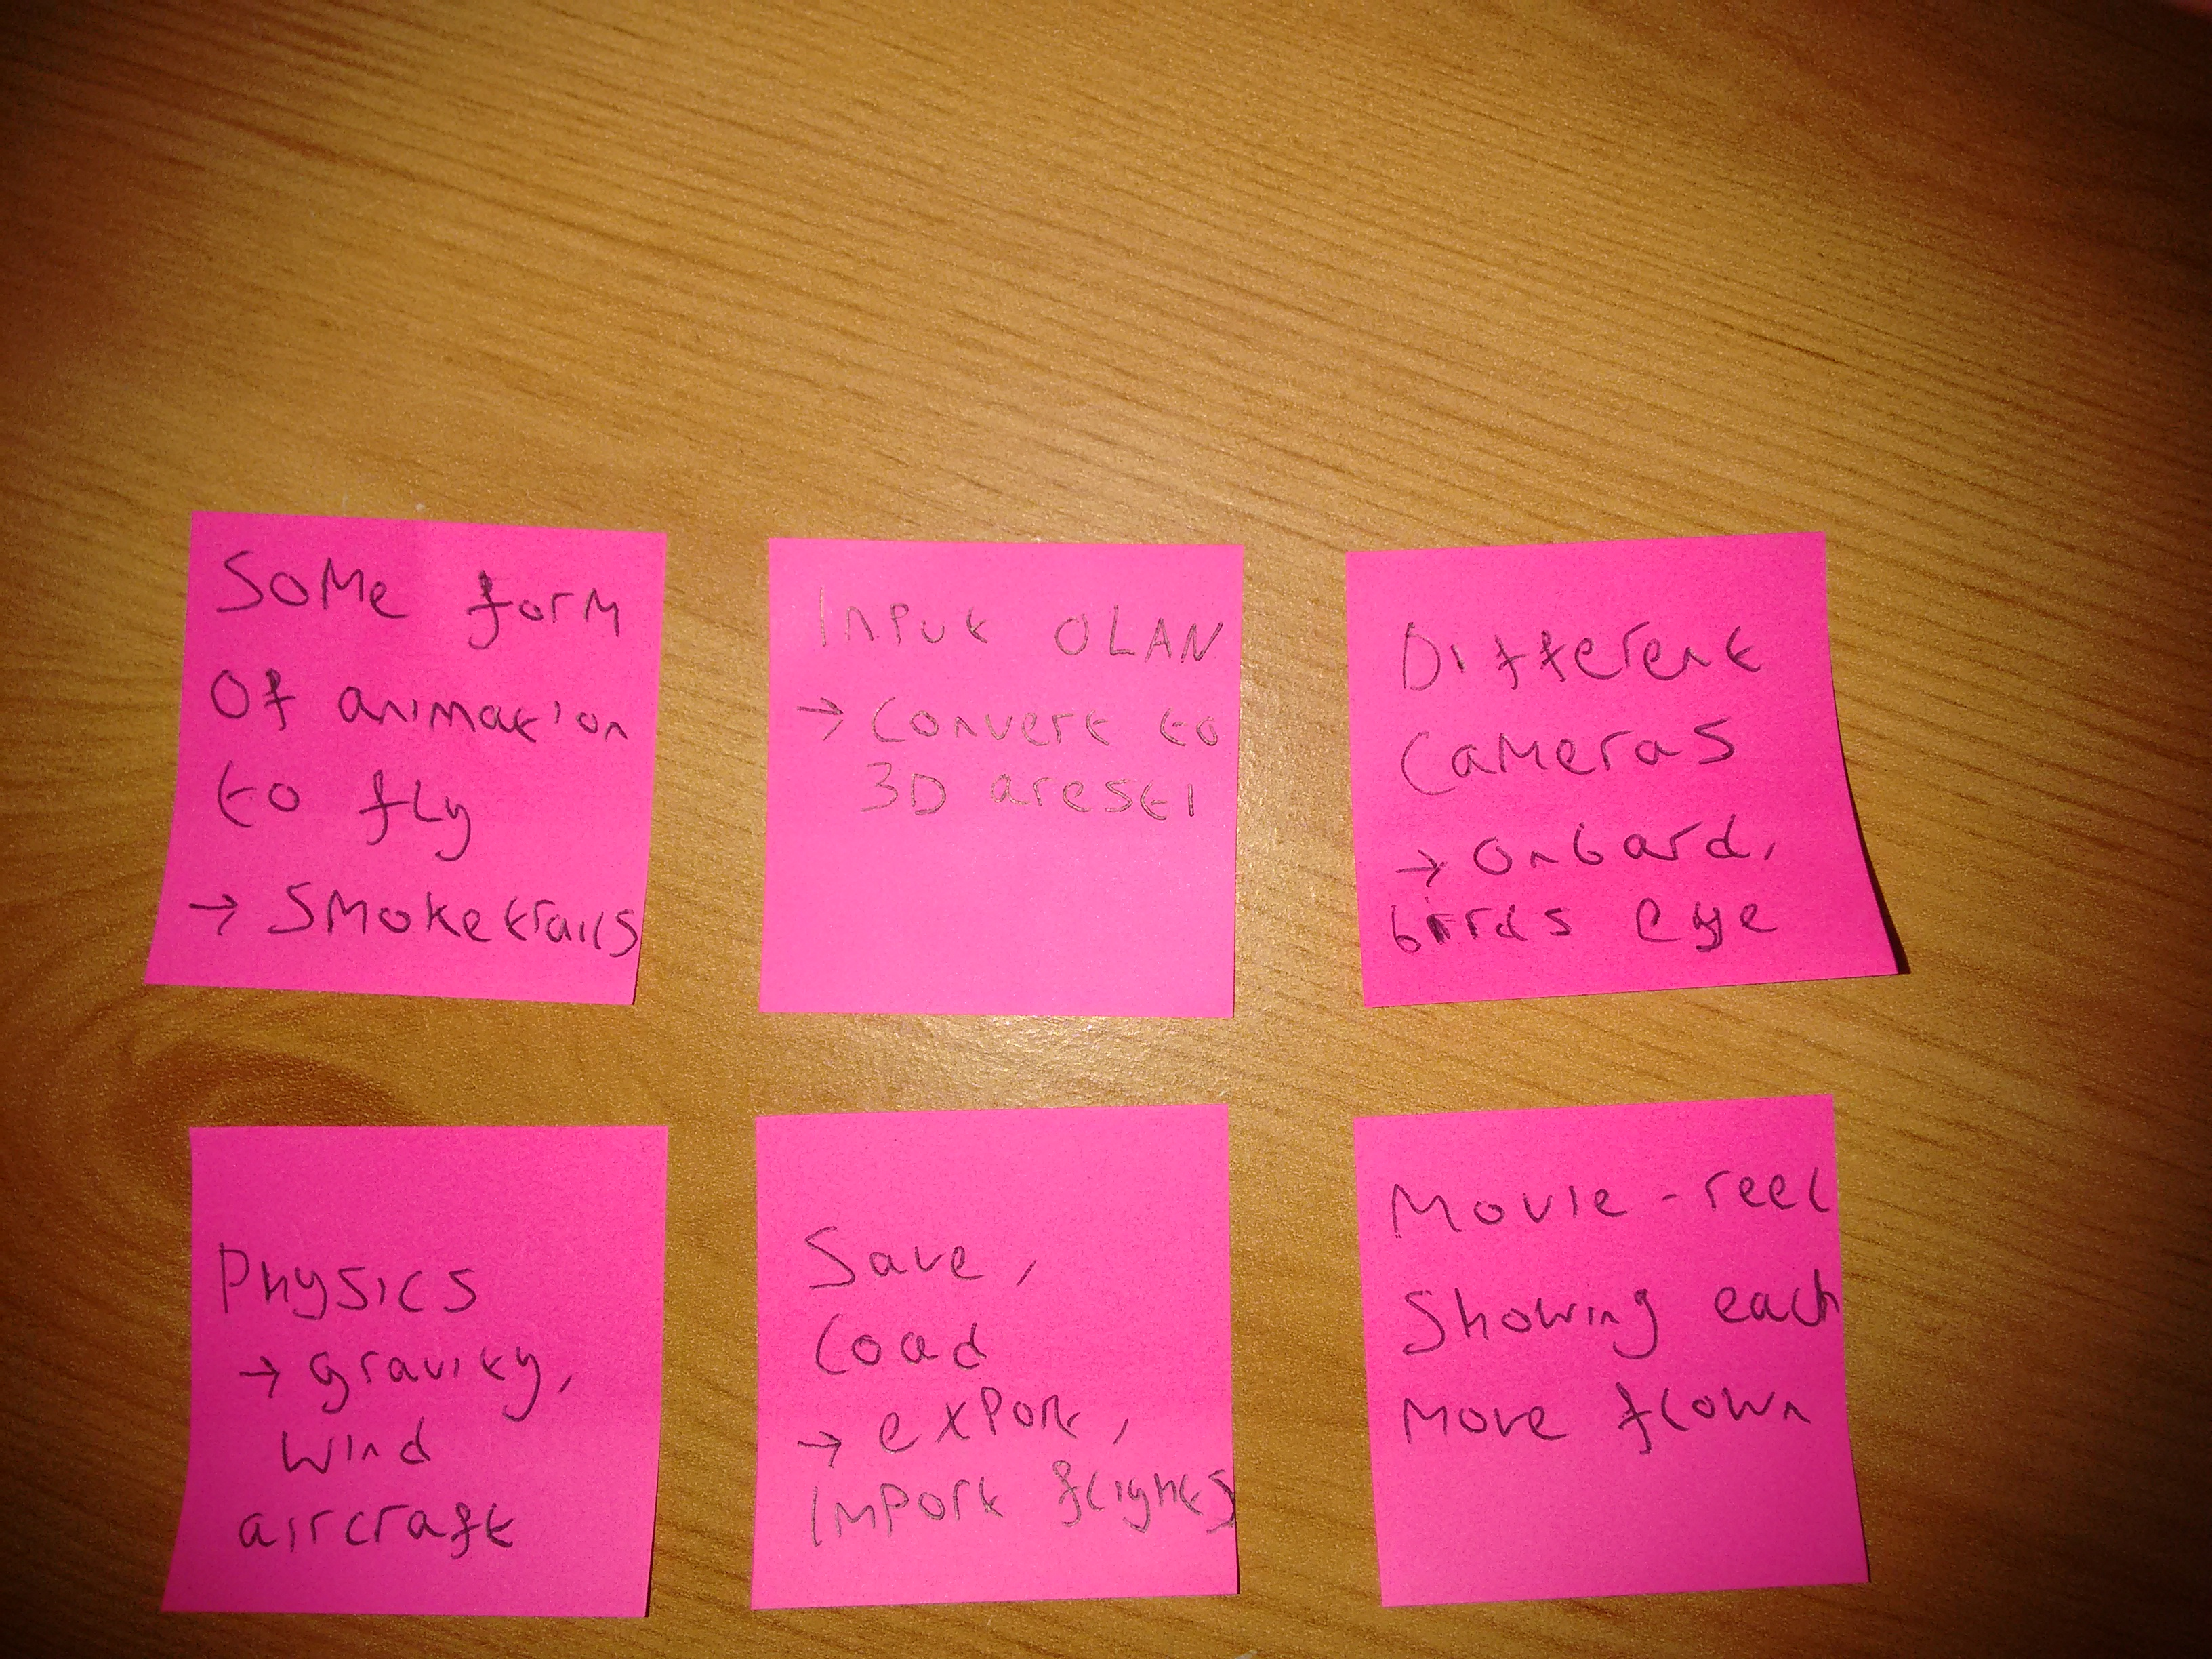
\includegraphics[width=0.5\textwidth]{images/notes.jpg}
  \caption{Image of the initial user stories after the first meeting, short and concise requirements.}
\end{figure}

\noindent The initial required application can be broken down into an extensive(but less detailed) list of main functional requirements. These are as follows:
\begin{enumerate}
	\item Provide a web-implemented tool that allows input of the OLAN 1 None-IE due to WebGL capabilities. Will it use a simple JSON file to store notations? characters as a string format, alongside possible click functionality.
	\item Relate each notation or set of notations to a certain procedural movement(rotations, movements etc.). 
		\begin{itemize}
			\item Must consider parameters in some of the notations, such as the speed of entry.
		\end{itemize}
	\item Provide a means of linking up these movements in such a way into moves, or the angle of the plane. They should produce a fluid manoeuvre.
	\item Display this using WebGL. Libraries to consider that could help. Begin by initially testing simple shapes to move and fly around, then add textures, and plane structure.
	\item Are libraries OK to use? with some of the movements:
		\begin{itemize}
			\item glMatrix- JavaScript library for helping with performing actions to matrices\cite{GlMatrix}
			\item ThreeJS- Another JavaScript library, good with handling cameras and different views\cite{ThreeJs}
		\end{itemize}
	\item Allow user to add different effects such as wind, gravity changes and other physics. Could be better to implement these last, as it will be easier to test pure functionality of rolls etc. first, then figure out natural physics.
	\item Add functionalities of different viewpoints(on-board views, side views) to application.
	\item Possibility to add function to save (using local storage?) users different sets of manoeuvres?
\end{enumerate}

The list shown above also has an accompanying report in section~\ref{app:init} of appendix A which was created after the first project meeting. This report includes the list of initial requirements, alongside footnotes, and also a detailing of the methodology and process that is planned to be followed. The document can be found in the appendices section of this report. 

In addition to the list, it is felt that it should be highlighted why and what language will be used to create the application. WebGL was chosen over OpenGL because of two reasons, the first being that the idea of being able to run an application such as this simply in a web browser is a good one, without the need for any compilers or platforms installed on the user's device. The other reason being that is that the author already has good experience using JavaScript, and this will help when it comes to the writing code, making sure the coding style is appropriate, and maximising any features it could bring to the application. JavaScript is a language with one of the most amounts of libraries on the web, meaning that the requirement to develop more specialised code is less. The final reasoning behind choosing JavaScript is because of the running times. Generally, JavaScript can compile and run quicker than other languages, and can also load into the users browser quickly. Because of this trait, it would be the best choice, otherwise the user would have to install locally onto their machine.

\section{Analysis}
Before beginning using the chosen life cycle model, It is important to analyse the overall model and requirements of the intended application. It is planned to analyse two items: the requirements analysed by time, effort and difficulty, and also a breakdown of the OLAN and Aresti manoeuvres. The second of which will be broken down to their primitive forms, hopefully finding out how the application can create each manoeuvre as simple and efficiently as possible.

\subsection{OLAN and Aresti interpretations}
The best place to begin with the analysis is to look in more detail at the OLAN manoeuvres individually, by breaking down each manoeuvre into their primitive elements. As with the previous section, alongside this section there an attached document to the appendices of this report, detailing the main and most important manoeuvres that are key to finding primitive shapes. This began by firstly organising each OLAN and their corresponding Aresti shapes into sub groups. 

Of these, there were:
\begin{itemize}
	\item Single element- These include manoeuvres that can be described as one fluid movement. For instance, the OLAN letter 'd' would mean diagonal line up, which requires only one action to complete the manoeuvre.
	\item Two-element- This group includes any manoeuvres that require two separate manoeuvres to complete a given manoeuvres. An example of this could be the 'z' notation, also known as a shark tooth. This shape requires both a diagonal line up followed by a vertical line down. 
	\item Loops- These like the single element moves, consist of a single manoeuvre, and can be combined to make other manoeuvres.
	\item Loop-line combinations- These are loops that are a combination of a loop and a single or two-element manoeuvre.
	\item Double-loops- As the name states, these are manoeuvres that contain two loops.
	\item Humpty-Dumpties, Hammerheads and Tailslides- Each of these manoeuvres represent specific shapes, such as a 'humpty dumpty' which consists of a bump shape comprised of a 180 degree turn to come back down vertically. As the previous, these shapes can simply be combined from single element pieces. 
	\item Complex 3 rolling elements- The naming behind this group of manoeuvres comes from the fact that each contain a set of 3 elements to create the entire figure.
	\item Special and 'oddball' figures- The group of manoeuvres that are more complex in such a way that they require special sections not available from any of the other groups. One example of this is the OLAN letter 'f' which represents a flick. This comprises of rolling the aircraft 360 degrees along its horizontal line.
\end{itemize}

Another important part of the OLAN analysis that had to be understood before proceeding was the possible parameters, prefixes and postfixes that can be attached to manoeuvres. 

Looking at prefixes first, each one-letter-notation, \textbf{some moves} are able to be reversed, or inverted. These are so:
\begin{itemize}
	\item r - Reverse, meaning to order of how each part of the manoeuvre is done. For example, placing the letter 'r' before 'c', would represent a Cuban loop flown in the opposite order. 
	\item i - Inverse, meaning that each part of the manoeuvre is done in the same order, but inverted in terms of value. For example, the letter 'i' before 'c' would mean that rather than looping upwards, the loop would go down. A diagonal line upwards would become a diagonal line downwards.
	\item ir - This is simply a mixture of both the previous. The manoeuvre fixed to the end of this postfix would both be inverted and then reversed. 
\end{itemize}

In addition, there are a number of postfixes that can be used with some manoeuvres particularly with roll or turn based figures. For example, manoeuvres containing rolls can be represented with the prefix angle of turn in multiples of 90 degrees, and a postfix of the amount of rolls along the same part of the path. So in one example, the notation '2j2' would represent a 180 degree turn, whilst rolling the aircraft twice. Alike the prefixes for inverting and reversing manoeuvres, the parameters are not available on all the manoeuvres in the OLAN catalogue. Again, the full list can be found on the the OpenArea site, or see the the OLAN understandings in section~\ref{app:olan} of appendix A.

One final set of optional parameters that could be required of the application to handle are the positions of manoeuvres. Although not strictly in part of the OLAN catalogue, it is already available in the OpenAero application. These parameters are structured (x,y) with x representing the amount of horizontal distance and y the vertical distance from the end of the previous manoeuvre to the start of the current manoeuvre. These can also be negative values to ensure the user can control the position fully. 

The main reason for the need of this is that simply all manoeuvres cannot fully follow each other straight after each other. In real-life if a manoeuvre made the pilot finish near the ground, and the next move required them to perform a diagonal line down, they would hit the ground. Obviously the application will attempt some form of validation and checks, but offering the option to the user is a very useful feature.

From analysis in the groups listed above, a number of assumptions can be made.
\begin{enumerate}
	\item it has already been deduced that all none-single manoeuvres that do not include loops or rolls should be possible to be made from a set of single element manoeuvres.
	\item In total, any manoeuvre can be constructed from one of three primary moves: diagonal and straight lines, curved lines, and turns and rolls. Each of which should be able to carry parameters.
	\item Each curve should be possible to be created based on 45 degree increments, as this is the smallest change of angle in any manoeuvre, and all other angles seem to be in multiples of this number. This will shorten the need for multiple commands for different ranges of angles when programming in the manoeuvres. Because the changes in angle will need to be by a curve, interpolation will be required to make the change in angle smooth and realistic.
	\item Turns, curves and rolls will all need parameters, as some curves are steeper and shorter than others. The same goes for rolls, where you can choose anything from quarter to 3 rolls, and in turns the angle of turn should be specifiable.
\end{enumerate}

By considering the analysis of the set of manoeuvres, it can now envision what manoeuvres will be possible to create easiest, and prioritise the work better. The next section of this report will group up the functionality of the application with the OLAN manoeuvre findings.

\subsection{Application functionality interpretations}
Upon having the initial meetings with the project supervisor, and on analysis of the OLAN catalogue, more final judgments can be made on what is desired to have been achieved by the end of this project. As discussed in the background section, a set of initial assumed requirements have already been created. Though, some of the features raised questions, such as the possibilities to use libraries for the physics and graphical side. After some research, a cohesive and stable list of features and requirements of the application can now be defined. Rather than in a list format though, features will be grouped together and discuss the most important factors. The use-case for the grouped together requirements can be seen in figure~\ref{fig:usereq}. Following the use-case is a ranked table~\ref{tbl:rank-table} of the requirements, in order of priority.


\begin{figure}[h!]
  \centering
      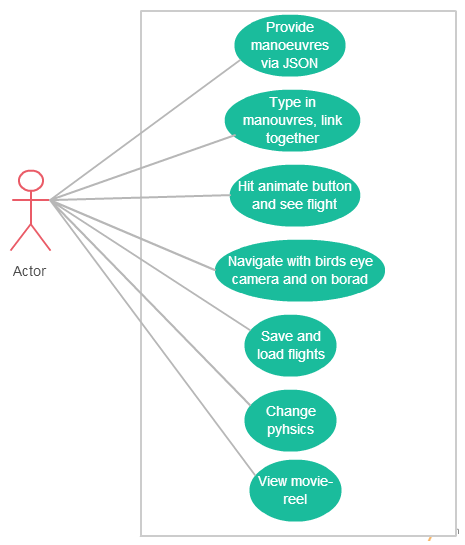
\includegraphics[width=0.8\textwidth]{images/usereq.png}
  \caption{Use-case of grouped requirements from initial research}
  \label{fig:usereq}
\end{figure}

\clearpage

\begin{table}[h!]
\caption{A table of prioritised features and tasks that would like to have implemented by the end of the project. The lower ranked items will only be started on completion of higher tasks.}
 \label{tbl:rank-table}
\begin{tabular}{|l|l|}
\hline
\textbf{Rank} & \textbf{Description}                                                                \\ \hline
1             & Support broken down manoeuvres, via JSON, convert to vectors and ultimately figures \\ \hline
2             & Allow for each manoeuvre to link together, start at end of previous                 \\ \hline
3             & Animate along a path of the manoeuvres                                              \\ \hline
4             & Create cameras, onboard and birds eye                                               \\ \hline
5             & Ground and lighting additions                                                       \\ \hline
6             & Saving and loading of inputs                                                        \\ \hline
7             & Manoeuvre validation                                                                \\ \hline
8             & Physics options, different aircrafts                                                \\ \hline
9             & Movie reel functionality                                                            \\ \hline
10            & Mobile compatibility and nice GUI                                                   \\ \hline
\end{tabular}
\end{table}

Starting with the underlying functionality based on the OLAN interpretations, what is hoped to have been achievable by the end of this project is the possibility to allow users to enter any length of space separated OLAN characters into an input box, alongside any possible prefixes, postfixes and parameters. Is is hoped to have achieved this by making the system as general as possible, and by using very abstract methods that can support any given move input. One way of implementing this now would be to break each manoeuvre into a set of instructions, each one saying which direction to move, the angle and length. By breaking each manoeuvre into these, a single method could be used to construct each manoeuvre on the fly. This is important as it would then allow for the user to play through the manoeuvre in an animated fashion and see the aircraft move.

More generally, one of the questions asked at the start of this project was if libraries could be used to help create the graphics and physics. By now, more meetings with the project supervisor have taken place and found this was allowable. The main library to have been considered after this has been the ThreeJS\cite{ThreeJs} library which acts as a good wrapper for controlling a wide range of objects in a scene. This library will allow vectors, cameras and lighting to be easily manipulated, which will form the basis of the application. A discussion of the use of this library when it comes to planning each of the features in the design will take place.

This will lead up to the scene and cameras that is hoped to be working to a good standard. For the scene, things such as the ground terrain are not so important, and can simply represent a flat land, while lighting could be added, but perhaps after fundamental features are added. As for cameras, it would be preferred that there is a set of two cameras: one for navigating and viewing flight paths at different locations and angles, and another camera which would be on-board, like a nose-cam.

The save/ loading of flight paths is a lower ranked task, but is something that will definitely be planned to have been implemented by the end of the project. Having looked into various methods of saving the OLAN entries, the best way that was found is to use a combination. One which would use local storage, and one that would export to JSON. The first of which was found out here\cite{Local_Storage} is particularly useful as the project is web based.

There are four features that would be useful to add, but these will be optional for now, and these may be added after the previously mentioned features. The first of which would be to validate the manoeuvre entry. Currently in the OpenAero application there is a check that looks how close and where manoeuvres are placed on the canvas, and for the application it would be ideal to have a check that looks if manoeuvres are actually possible from the current rotation or placement of the last manoeuvres ending position. Another big check would be if the current path of the aircraft was to hit the floor, a check should be made.

Physics is also an option that would preferably be included, such as wind, type of aircraft(each aircraft could be more difficult to navigate corners, meaning wider curves). And relating back to the function of playing the animation once the manoeuvres are drawn, an idea given from the project supervisor was of a 'movie-reel' function that would show a mini image of the current manoeuvre being played, showing the animation progressing through each one. Again, this is another feature that would be prioritised less, and implemented after other key features.

Finally, a smaller task that could be performed is to make the application mobile compatible. As most phones also now have WebGL capabilities, making the application run on mobiles should be possible. This is more a GUI centred feature on the site itself though, and should be added nearer the end of the project.

\section{Process}
Moving onto more project and time management specific items, the process which is followed can have a large effect on what features are complete on time. At this stage, it is suggested that a hybrid of both the waterfall methodology alongside feature-driven development is used to create the application. The reasoning for this starts with the way a list of features in the analysis has already been created, which is already part of the FDD life cycle. This would mean by following this, it  would be possible to simply iterate over each feature, plan, implement and test one by one. This is an ideal trait that comes from using this methodology which allows the creation of each feature separately, and more importantly by priority. Then for instance if the entire list outlined was not finished, the application would still have a good deal of functionality on offer. A guide found on the agile modelling site\cite{FDD} explained backed this up, and explained FDD to a good understanding. If the waterfall method was used alone, It might mean that too many items are implemented at once, even though some features rely on others completed. This would result in an incomplete and less functional program. There is also a clear part of the scrum methodology put to use here, as it is showed with some user stories, and the prioritised list of features.

The second reason, and reason for including the waterfall cycle in this hybrid approach is because it would it would allow the creation of a more big up front design before beginning implementation. This is where this approach is going to be different from a solely FDD way, where it would usually require having to design each feature before implementation and testing. In some opinions, this is because of the preference of knowing how the entirety of the structure of code should look before it is begun, yet keeping the structure as loosely connected as possible to ensure that features avoid relying on each other to an extent where if one is broken, the rest is broken. 

Because the methodology has been chosen in this fashion, it has meant a Gantt chart based on stages of planning and design has been created, and also what features are hoped to have been accomplished at times throughout the project. This, coupled with a work blog, will allow is to be possible to track progress throughout, and compromise when time is needed, or move along the list of features if time is available. The Gantt chart will be updated as time progresses in relation to the blog, where it will then be possibleto see where progress is up to overall.

As for implementation and testing, these will be carried out in the FDD way by implementing and testing each feature one at a time. In the implementation stage of each, it will be ensured that decoupling is a priority meaning that any developing code does not damage any current working functionality of another feature. The implementation and testing schedules of each feature can be seen on the updated Gantt chart in section~\ref{app:gantt2} of appendix A. This time, the Gantt chart tasks in to consideration the difficulty and time required to implement and test each feature.